\documentclass[aspectratio=169]{ctexbeamer}
\definecolor{urls}{RGB}{137, 180, 250}
\definecolor{link_text}{RGB}{245, 224, 220}
\hypersetup{
  colorlinks,
  linkcolor=, % This config controls the jumps inside the pdf
  urlcolor=urls,
}
\renewcommand{\UrlFont}{\ttfamily\scriptsize}

\usetheme{AnnArbor}
\usepackage[style=Mocha,accent=Rosewater]{beamercolorthemecatppuccin}

\usefonttheme{serif}
\usefonttheme{professionalfonts}

\usepackage[T1]{fontenc}
\setmainfont{LXGW WenKai}
% \setmainfont{Cascadia Code NF}
% \setsansfont{}
\setmonofont{Cascadia Code NF}
\usepackage{xeCJK}
\setCJKmainfont{LXGW WenKai}
% \setCJKmainfont{}
\setCJKmonofont{Cascadia Code NF}
\newcommand{\nerd}[1]{\texttt{#1}}
\setmonofont{Cascadia Code NF}[
  Contextuals=Alternate
]

\PassOptionsToPackage{hyphens}{url}
% \usepackage{ulem}
\usepackage{graphicx}
%\usepackage{wrapfig}
\usepackage{pifont} % Symbols used as itemize symbols
\usepackage{enumitem}
\setlist[itemize,1]{label={\small\color[RGB]{242, 205, 205}\ding{111}}}
\setlist[itemize,2]{label={\footnotesize\color[RGB]{242, 205, 205}\ding{111}}}
\setlist[itemize,3]{label={\scriptsize\color[RGB]{242, 205, 205}\ding{111}}}
\usepackage{float}
\usepackage{booktabs}

\setbeamerfont{footnote}{size=\tiny}
\setbeamertemplate{footnote}{%
  \color[RGB]{108, 112, 134}%
  \insertfootnotetext%
}
\setlength{\footnotesep}{0.3\baselineskip}
\newcommand{\refnote}[1]{\footnotetext{#1}}

\usetheme{AnnArbor}

\usepackage{amsmath, amssymb, amsthm}
\usepackage{listings}
\lstdefinestyle{bash}{
  alsoletter=-,
  keywordstyle=[2]{\color[RGB]{243, 139, 168}},
  morekeywords=[2]{sudo},
  keywordstyle=[3]{\color[RGB]{166, 227, 161}},
  morekeywords=[3]{add-apt-repository, apt-get, apt},
  keywordstyle=[4]{\color[RGB]{250, 179, 135}},
  morekeywords=[4]{install},
}
\lstdefinestyle{lua}{
  alsoletter=-,
  keywordstyle=[2]{\color[RGB]{137, 180, 250}},
  morekeywords=[2]{name, priority, opts, config, dependencies, submodules, main, version, init, number, boolean, event},
  keywordstyle=[3]{\color[RGB]{180, 190, 254}},
  morekeywords=[3]{fun, setup},
  keywordstyle=[4]{\color[RGB]{250, 179, 135}},
  morekeywords=[4]{},
}
\lstdefinestyle{path}{
  alsoletter=~,
  basicstyle={\footnotesize\ttfamily\color[RGB]{147, 153, 178}\itshape},
}
\lstset{
  language={[5.1]lua},
  style=lua,
  basicstyle=\footnotesize\ttfamily,
  breaklines=true,
  showstringspaces=false,
  breakatwhitespace=true,
  keywordstyle=\color[RGB]{245, 169, 127},
  numberstyle={\ttfamily\color[RGB]{110, 115, 141}},
  commentstyle={\color[RGB]{147, 153, 178}\itshape},
  stringstyle={\color[RGB]{166, 218, 149}},
}
% NOTE: \lstinline{} command does not support background color
\lstdefinestyle{nvim}{
  alsoletter=:,
  keywordstyle=[3]{\color[RGB]{166, 227, 161}},
  morekeywords=[3]{:Tutor, :help, :checkhealth}, % ChkTeX 26
  keywordstyle=[4]{\color[RGB]{250, 179, 135}},
  morekeywords=[4]{snacks},
}

\newcommand{\TODO}[1]{\textcolor{red}{TODO\@: #1} }

% \newcommand{\link}[3][]{\href{#3}{#2}\footnote[#1]{\url{#3}}}
\newcommand{\link}[3][]{\href{#3}{#2\textsuperscript{\nerd{}}}}



\title{Neovim从入门到出门}
\subtitle{第五节:代码编辑(一)}
\author{Jacky-Lzx}
\date{\today}

\usepackage{tikz}
\titlegraphic {
  \begin{tikzpicture}[overlay,remember picture]
    \node at (-6, 4.5){
      
\includegraphics[height=1cm]{./Figures/Neovim_logo.png}
    };
    \node at (6, 4.5){
      
\includegraphics[height=1cm]{./Figures/Catppuccin_logo.png}
    };
  \end{tikzpicture}
}

\usepackage{makecell}

\begin{document}

\begin{frame}
  \titlepage
\end{frame}

\begin{frame}{大纲}
  \tableofcontents
\end{frame}
% Current section
\AtBeginSection[ ] {
  \begin{frame}{大纲}
    \tableofcontents[currentsection]
  \end{frame}
}

% TODO: 记得检查catppuccin的插件是否添加

\section{问题反馈}
  \begin{frame}[fragile]{问题反馈}

    \begin{itemize}
      \item 问题\\
        \begin{figure}[H]
          \centering
          
\includegraphics[width=0.8\linewidth]{./Figures/Issue.jpg}
        \end{figure}
      \item 修改\\
        \begin{itemize}
          \item 把
            \begin{lstlisting}[basicstyle=\tiny\ttfamily]
    vim.keymap.set({ "n", "x" }, "<S-H>", "^", { desc = "Start of line" })
    vim.keymap.set({ "n", "x" }, "<S-L>", "$", { desc = "End of line" })
    vim.keymap.set("n", "y<S-H>", "y^", { desc = "Yank from start of line" })
    vim.keymap.set("n", "y<S-L>", "y$", { desc = "Yank to end of line" })
            \end{lstlisting}
            改成
            \begin{lstlisting}[basicstyle=\tiny\ttfamily]
    vim.keymap.set({ "n", "x", "o" }, "<S-H>", "^", { desc = "Start of line" })
    vim.keymap.set({ "n", "x", "o" }, "<S-L>", "$", { desc = "End of line" })
            \end{lstlisting}
        \end{itemize}
    \end{itemize}
  \end{frame}

\section{插件安装和配置}

  \subsection{nvim-autopairs}
    \begin{frame}[fragile]{\link{nvim-autopairs}{https://github.com/windwp/nvim-autopairs}:自动关闭括号}

      \begin{lstlisting}
  {
    "windwp/nvim-autopairs",
    event = "InsertEnter",
    opts = {
      ignored_next_char = "[%w%.]", -- will ignore alphanumeric and `.` symbol
    },
  },
      \end{lstlisting}
    \end{frame}

  \subsection{trim.nvim}
    \begin{frame}[fragile]{\link{trim.nvim}{https://github.com/cappyzawa/trim.nvim}:在保存时删除行后空格}

      \begin{lstlisting}
  {
    "cappyzawa/trim.nvim",
    event = "BufWritePre",
    opts = {},
  },
      \end{lstlisting}

    \end{frame}

  \subsection{undotree}
    \begin{frame}[fragile]{\link{undotree}{https://github.com/jiaoshijie/undotree}:保存文件的历史版本}

      \begin{lstlisting}[basicstyle=\tiny\ttfamily]
  {
    "mbbill/undotree",
    keys = {
      { "<leader>ut", "<cmd>UndotreeToggle<cr>", desc = "Toggle undo-tree" },
    },
    init = function()
      vim.cmd([[
      if has("persistent_undo")
         let target_path = expand('~/.undodir')

          " create the directory and any parent directories if the location does not exist.
          if !isdirectory(target_path)
              call mkdir(target_path, "p", 0700)
          endif

          let &undodir=target_path
          set undofile
      endif
      ]])
    end,
  },
      \end{lstlisting}
    \end{frame}

  \subsection{Comment.nvim}
    \begin{frame}[fragile]{\link{Comment.nvim}{https://github.com/numToStr/Comment.nvim}:快速注释代码}

      \begin{lstlisting}[basicstyle=\tiny\ttfamily]
  {
    "numToStr/Comment.nvim",
    keys = {
      { "<leader>/", function() require("Comment.api").toggle.linewise.current() end,                 mode = "n", desc = "[Comment] Comment current line", },
      { "<leader>/", "<esc><cmd>lua require('Comment.api').toggle.linewise(vim.fn.visualmode())<cr>", mode = "v", desc = "Comment current line",           },
      -- control + / keymappings
      { "<C-_>",     function() require("Comment.api").toggle.linewise.current() end,                 mode = "n", desc = "[Comment] Comment current line", },
      { "<C-_>",     "<esc><cmd>lua require('Comment.api').toggle.linewise(vim.fn.visualmode())<cr>", mode = "v", desc = "Comment current line",           },
    },
    config = true,
  },
      \end{lstlisting}
    \end{frame}

  \subsection{smartyank.nvim}
    \begin{frame}[fragile]{\link{smartyank.nvim}{https://github.com/ibhagwan/smartyank.nvim}:自动复制到系统剪切板}

      \begin{lstlisting}
  {
    "ibhagwan/smartyank.nvim",
    event = { "BufWinEnter" },
    opts = {
      highlight = {
        timeout = 500, -- timeout for clearing the highlight
      },
      clipboard = {
        enabled = true,
      },
      osc52 = {
        silent = true, -- true to disable the "n chars copied" echo
      },
    },
  },
      \end{lstlisting}
    \end{frame}

  \subsection{flash.nvim}
    \begin{frame}[fragile]{\link{flash.nvim}{https://github.com/folke/flash.nvim}:快速跳转}

      \begin{lstlisting}[basicstyle=\tiny\ttfamily]
  {
    "folke/flash.nvim",
    event = "BufReadPost",
    opts = {
      label = { rainbow = { enabled = true, shade = 1 } },
      modes = { char = { enabled = false } }
    },
    keys = {
      { "<leader>f", mode = { "n", "x", "o" }, function() require("flash").jump() end,              desc = "[Flash] Jump"              },
      { "<leader>F", mode = { "n", "x", "o" }, function() require("flash").treesitter() end,        desc = "[Flash] Treesitter"        },
      { "<leader>F", mode = { "o", "x" },      function() require("flash").treesitter_search() end, desc = "[Flash] Treesitter Search" },
      -- ...
    },
  },
      \end{lstlisting}

    \end{frame}

  \subsection{todo-comments.nvim}
    \begin{frame}[fragile]{\link{todo-comments.nvim}{https://github.com/folke/todo-comments.nvim}:高亮显示TODO项目}

      \begin{lstlisting}
  {
    "folke/todo-comments.nvim",
    dependencies = {
      "nvim-lua/plenary.nvim",
      "folke/snacks.nvim"
    },
    event = "VeryLazy",
    keys = {
      { "<leader>st", function() require("snacks").picker.todo_comments({ keywords = { "TODO", "FIX", "FIXME", "BUG", "FIXIT", "HACK", "WARN", "ISSUE"  } }) end, desc = "[TODO] Pick todos (without NOTE)", },
      { "<leader>sT", function() require("snacks").picker.todo_comments() end, desc = "[TODO] Pick todos (with NOTE)", },
    },
    config = true,
  },

      \end{lstlisting}

    \end{frame}

  \subsection{mini.surround}
    \begin{frame}[fragile]{\link{mini.surround}{https://github.com/echasnovski/mini.surround}:快速添加、删除括号}

      \begin{lstlisting}
  {
    "echasnovski/mini.surround",
    version = "*",
    event = "BufReadPost",
    config = true,
    keys = {
      -- Disable the vanilla `s` keybinding
      { "s", "<NOP>", mode = { "n", "x", "o" } },
    },
  },
      \end{lstlisting}
    \end{frame}

  \subsection{mini.ai}
    \begin{frame}[fragile]{\link{mini.ai}{https://github.com/echasnovski/mini.ai}:textobject拓展}

      \begin{lstlisting}
  {
    -- Extend `a`/`i` textobjects
    "echasnovski/mini.ai",
    version = "*",
    event = "BufReadPost",
    config = true,
  },
      \end{lstlisting}

    \end{frame}

  \subsection{multicursor.nvim}
    \begin{frame}[fragile]{\link{multicursor.nvim}{https://github.com/jake-stewart/multicursor.nvim}:多光标}

      \begin{lstlisting}[basicstyle=\tiny\ttfamily]
  {
    "jake-stewart/multicursor.nvim",
    branch = "1.0",
    event = "BufReadPost",
    keys = {
      -- Append/insert for each line of visual selections. Similar to block selection insertion.
      {"mI", function() require("multicursor-nvim").insertVisual() end, mode = "x", desc = "Insert cursors at visual selection"},
      {"mA", function() require("multicursor-nvim").appendVisual() end, mode = "x", desc = "Append cursors at visual selection"},
    },
    config = function()
      local mc = require("multicursor-nvim")
      mc.setup()

      -- Mappings defined in a keymap layer only apply when there are multiple cursors. This lets you have overlapping mappings.
      mc.addKeymapLayer(function(layerSet)
        -- Enable and clear cursors using escape.
        layerSet("n", "<esc>", function()
          mc.clearCursors()
        end)
      end)

    end,
  },
      \end{lstlisting}
    \end{frame}

  \subsection{vim-wakatime}
    \begin{frame}[fragile]{\link{vim-wakatime}{https://wakatime.com}:编程时间统计} % ChkTeX 19

      \begin{lstlisting}
  { "wakatime/vim-wakatime", lazy = false },
      \end{lstlisting}

      \begin{figure}[H]
        \centering
        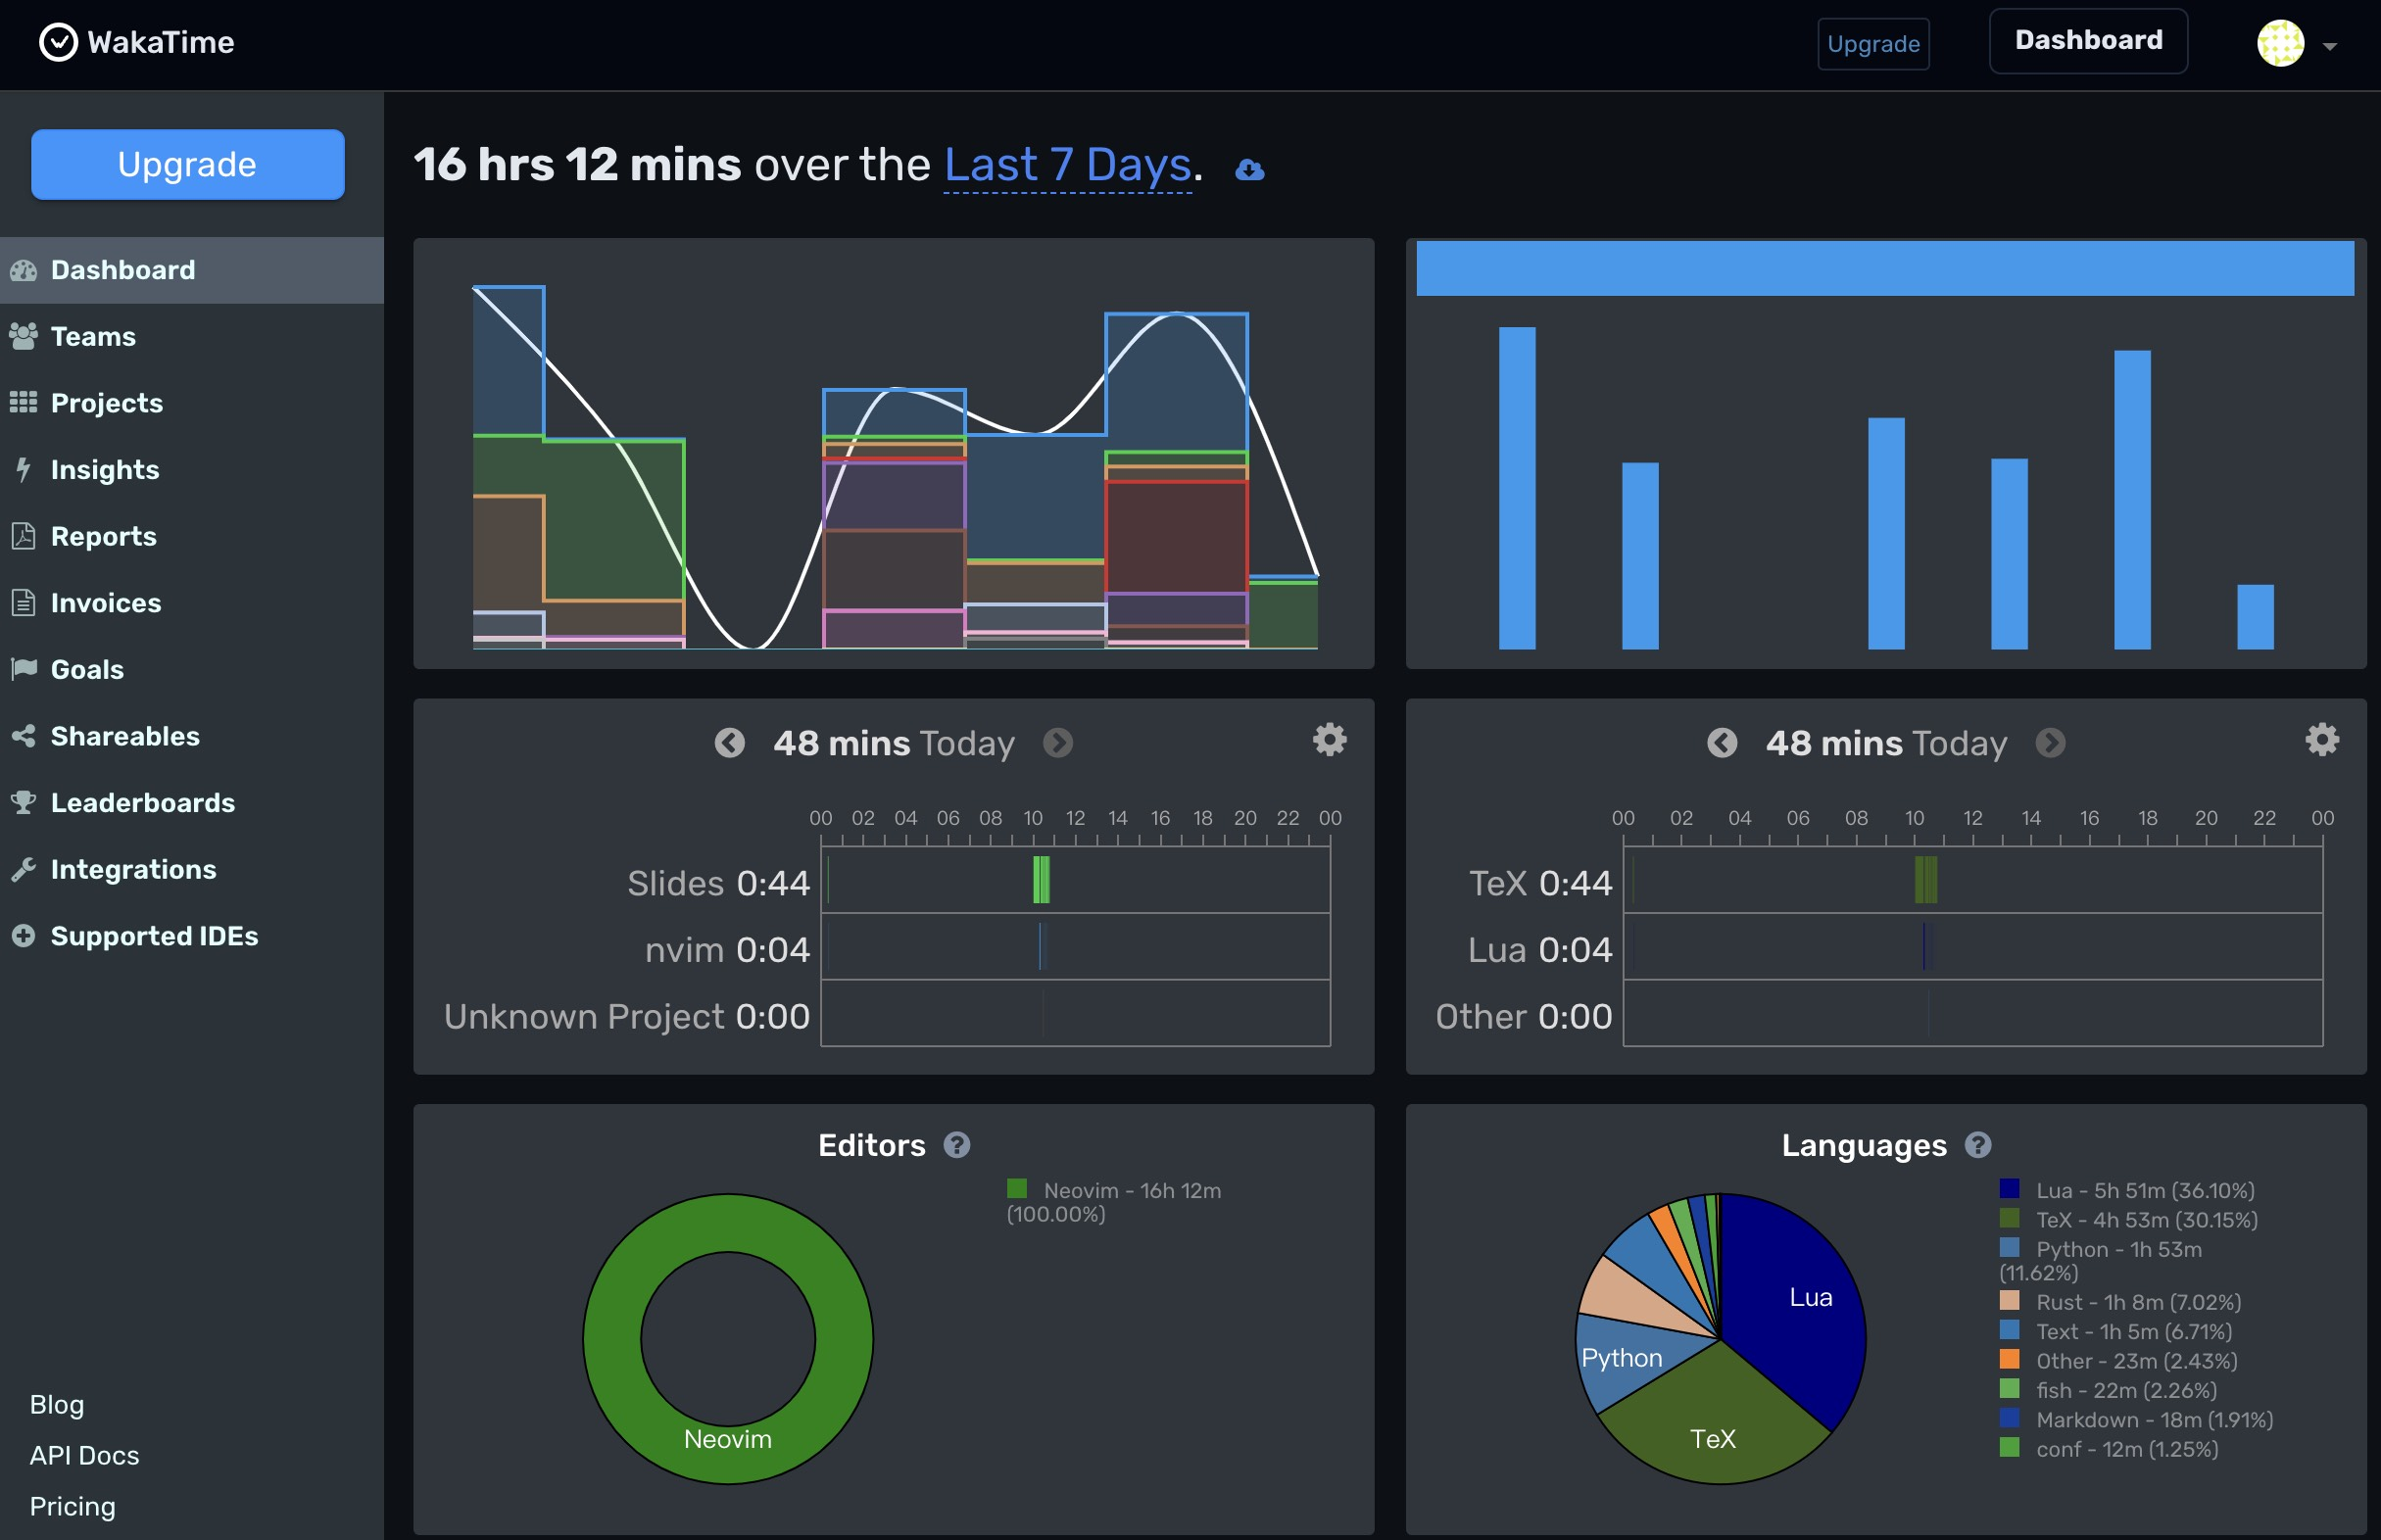
\includegraphics[width=0.6\linewidth]{./Figures/Wakatime.jpg}
      \end{figure}

    \end{frame}

    \begin{frame}
      \begin{itemize}
        \item 感谢:
          \begin{itemize}
            \item \link{Catppuccin}{https://catppuccin.com/} 
\includegraphics[height=10pt]{./Figures/Catppuccin_logo.png}
            \item \link{Catppuccin for beamer}{https://github.com/atticus-sullivan/beamercolortheme}
          \end{itemize}
          \vspace{0.5cm}
        \item 本教程的全部材料可以在我的Github上找到
          \begin{itemize}
            \item Slides: \url{https://github.com/Jacky-Lzx/nvim.tutorial.slides}
            \item Config: \url{https://github.com/Jacky-Lzx/nvim.tutorial.config}
          \end{itemize}
      \end{itemize}
    \end{frame}

\end{document}
